\documentclass[11pt]{article}

%####### DON'T CHANGE MARGIN SETTINGS ###########
\newcommand{\keywordfont}{\textsc}
\newcommand{\keyword}[1]{%
  \marginpar{\raggedright\small\keywordfont{#1}}}
\reversemarginpar
\usepackage[a4paper, top=2.5cm, bottom=2.5cm, outer=2cm, inner=3.3cm, marginparwidth=72pt, heightrounded]{geometry}
%#################################

\usepackage{amsmath}
\usepackage{amssymb}
\usepackage{hyperref}
\usepackage{graphicx}
\usepackage{microtype}
\usepackage{mathtools}

\begin{document}

\Large
\begin{center}
\textbf{MA3K7 Week $6/7$ Rubric}
\\
Timothy Yap (2161367)
\end{center}
\normalsize



%-----------------------------------------------------------------------------------------------------------

% Hat Numbers

% A hat contains 2024 pieces of paper numbered 1 through 2024. I draw two pieces of paper at random from the hat. The smaller of the two numbers drawn is subtracted from the larger. That difference is written on a new piece of paper which is placed in the hat, and the two original pieces are discarded. I repeat this process until one piece of paper remains. 

% What can you tell about the final piece of paper?

\section{Entry} %-------------------------------------------------------------------------------------------



We start with \keyword{I know} our hat and 2024 pieces of paper numbered 1 through 2024. After following the instructions, we end with one final piece of paper with a value. The absolute difference of any combination of two pieces of paper will be between 0 and 2024, so the value on our final piece of paper will be as well.

We will call \keyword{Introduce} the number on the final piece of paper the \textit{final value or final number} as above. Before listing out what else we know, we first want introduce  the idea of an \textit{iteration}. \\
An iteration is as follows: \\
\textbf{Step 1 -} Remove two pieces of paper. \\
\textbf{Step 2 -} Subtract the smaller of the two numbers from the larger one. \\
\textbf{Step 3 -} Add a new piece of paper with the value gotten from \textbf{Step 2} into the hat. \\
\textbf{Step 4 -} Repeat until one piece of paper remains. This is our final value. 
The last iteration is where we get our final value, the key to this investigation. We will also introduce the notion of \textit{size} $n$, which is just the initial amount of paper in our hat. 

    We also know \keyword{I know} the following:
\begin{itemize}
    \item The final value will be an integer.
    \item There will be $n-1$ iterations; 2023 iterations based on our initial set of parameters.
    \item Step 2 of our iteration is the same as finding the absolute difference of two numbers.
\end{itemize}

I want to \keyword{I want} explore the following questions:
\begin{itemize}
    \item What value will we get for our final piece of paper?
    \item Are there any values we can not obtain?
    \item Does our starting conditions affect this value?
\end{itemize}

We can try \keyword{Try} to generate a number using a smaller hat, say of size $n=4$ but we first introduce \keyword{Introduce} the following notation. The values in our hat will be shown in set notation, e.g. $\{1,2,3\}$. An iteration will be shown by an arrow, where the pair above shows Step 1 of our iteration recipe.
Below shows how one may arrive at a final value.

\[
\{1, 2, 3, 4\} \ \xrightarrow[|1-2|=1]{(1,2)} \ \{1, 3, 4\} \ \xrightarrow[|1-3|=2]{(1,3)} \ \{2, 4\}  \ \xrightarrow[|2-4|=2]{(2,4)} \ \{2\}
\]

%\keyword{Assumptions} 



%-----------------------------------------------------------------------------------------------------------

\section{Attack} %------------------------------------------------------------------------------------------



We can try \keyword{Strategic Specialisation} finding a final value for a smaller hat. Just by doing some by hand. We try $n=1,2,3$: 

\[
\{1\}
\]
\[
\{1, 2\} \ \xrightarrow[|1-2|=1]{(1,2)} \ \{1\}
\]
\[
\{1, 2, 3\} \ \xrightarrow[|1-2|=1]{(1,2)} \ \{1, 3\} \ \xrightarrow[|1-3|=2]{(1,3)} \ \{2\} , \hspace{20pt}
\{1, 2, 3\} \ \xrightarrow[|1-3|=2]{(1,3)} \ \{2, 2\} \ \xrightarrow[|2-2|=0]{(2,2)} \ \{0\} 
\]
\[
\{1, 2, 3\} \ \xrightarrow[|2-3|=1]{(2,3)} \ \{1, 1\} \ \xrightarrow[|1-1|=0]{(1,1)} \ \{0\}
\]

 While calculating these by hand we notice that the pair chosen does not matter. This lowers the amount of calculations that need to be done and is the reason why there is only 1 pair shown in $n=2$. For $n=3$, we had 6 permutations but only 3 unique pairs. Moving up to $n=2024$ \keyword{Stuck} will be extremely time-consuming to do by hand so we can implement this into Python to find our solution. Before going straight to $n=2024$, we continue with our \keyword{Try} strategic specialisation and try $n=4,5,6,\dots,20$ and writing all unique final values and the number of values into the following table:

\begin{table}[h]
    \centering
    \begin{tabular}{c|c|c|c|c|c} 
         $n$&  Final Values&  \# of Values&  $n$&  Final Values& \# of Values\\ 
         \hline
         1&  1&  1&  11&  0, 2, 4, 6, 8, 10& 6\\ 
         2&  1&  1&  12&  0, 2, 4, 6, 8, 10, 12& 7\\ 
         3&  0, 2&  2&  13&  1, 3, 5, 7, 9, 11, 13& 7\\ 
         4&  0, 2, 4&  3&  14&  1, 3, 5, 7, 9, 11, 13& 7\\ 
         5&  1, 3, 5 &  3&  15&  0, 2, 4, 6, 8, 10, 12, 14& 8\\ 
         6&  1, 3, 5&  3&  16&  0, 2, 4, 6, 8, 10, 12, 14, 16& 9\\ 
         7&  0, 2, 4, 6&  4&  17&  1, 3, 5, 7, 9, 11, 13, 15, 17& 9\\ 
         8&  0, 2, 4, 6, 8&  5&  18&  1, 3, 5, 7, 9, 11, 13, 15, 17& 9\\ 
         9&  1, 3, 5, 7, 9&  5&  19&  0, 2, 4, 6, 8, 10, 12, 14, 16, 18& 10\\
        10&  1, 3, 5, 7, 9& 5& 20& 0, 2, 4, 6, 8, 10, 12, 14, 16, 18, 20& 11\\ 
    \end{tabular}
\end{table}

We begin to \keyword{AHA} see some patterns! Firstly and obviously, the larger the $n$ the larger the number of unique final values. Secondly, the number of unique values is always less than or equal to $\frac{n}{2}+1$. Where equality only happens when $n$ is a multiple of 4, which is a pattern that hopefully fits with 2024.  Another observation is that the final values are always only odd or even. Furthermore, when $n \equiv 1 \text{ mod } 4$ or $n \equiv 2 \text{ mod } 4$, then the values are odd, and when  $n \equiv 0 \text{ mod } 4$ or  $n \equiv 3 \text{ mod } 4$, then the values are even. Lastly, if we plot the number of values, we can see a pattern emerge; $n \equiv 0 \text{ mod } 4$ has $\frac{n}{2}+1$ unique values, $n \equiv 3 \text{ mod } 4$ has $\frac{n + 1}{2}$ unique values, and when  $n \equiv 1 \text{ mod } 4$ or $n \equiv 2 \text{ mod } 4$, then there are $\frac{n + 1}{2}$ or $\frac{n}{2}$ unique values respectively. All these patterns \keyword{Generalise} are shown in the following table:

\begin{table}[h]
    \centering
    \begin{tabular}{c|c|c}
         Modulo Class&  Odd or Even Values&Number of Values\\
         \hline
         $n \equiv 1 \text{ mod } 4$&  Odd& $\frac{n + 1}{2}$\\
         $n \equiv 2 \text{ mod } 4$&  Odd&$\frac{n}{2}$\\
         $n \equiv 3 \text{ mod } 4$&  Even&$\frac{n + 1}{2}$\\
         $n \equiv 0 \text{ mod } 4$&  Even&$\frac{n}{2}+1$\\
    \end{tabular}
    \caption{Classification based on modulo 4}
    \label{tab:my_label}
\end{table}

This discovery leads to our first conjecture: \keyword{Conjecture} If $n \equiv 1 \text{ mod } 4$ or $n \equiv 2 \text{ mod } 4$ then the value of the final number is odd, otherwise it is even.
 
We can see the pattern holds for $n = 1,2,\dots,20$ \keyword{Justify} but to generalise we must first notice that in the case that our values are odd, there is an odd number of odd pieces of paper, and in the even case, we have an even number of odd pieces of paper. Another piece of information to note is the following:

\begin{table}
    \centering
    \begin{tabular}{c|c|c}
         First Piece of Paper &  Second Piece of Paper & Difference\\
         \hline
        Odd & Odd & Even\\
        Even & Even & Even\\
        Odd & Even & Odd\\
    \end{tabular}
    \caption{Difference of Pairs}
    \label{tab:my_label}
\end{table}

From above, we have two cases: a hat with $0 \text{ mod } 2$ (even case) pieces of paper with odd values or  $1 \text{ mod } 2$ (odd case) pieces of paper with odd values. Now using our table, if we are to find the difference between two values that are either both odd or even, then we either remove two odd numbers, that still leave us in same case or remove two even numbers, which don't affect the number of odd pieces of paper. Lastly, if we take one odd valued and one even valued piece of paper, then we still have the same number of odd pieces of paper. Thus in all scenarios, the number of odd pieces of papers stays the same. If we iterate this process to its ultimate conclusion, we get left with either an odd or even final value depending if our hat had an odd or even amount of odd valued pieces of paper. 

With this in mind, we see that the unique values are just all the odd or even values up to $n$. Which also gives us the following graph:

\begin{figure}[h] 
   \centering
   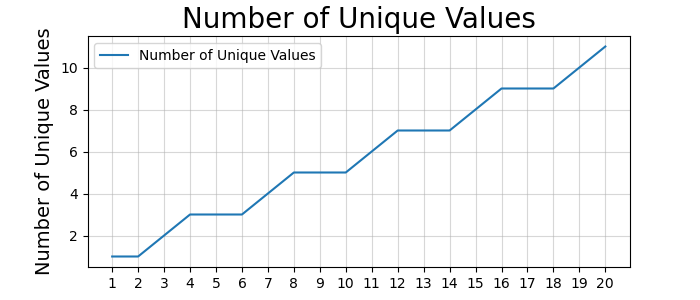
\includegraphics[width=5in]{graph.png}
   \label{myfig}
\end{figure}

Checking \keyword{Check} using Python, this pattern holds up to $n=80$. As every subsequent $n$ takes exponentially longer, we decide to cut it off there. Besides, this is enough to see that the pattern holds. So returning to our initial hat of $n=2024$, we know that $2024 \equiv 0 \text{ mod } 4$ so 2024 has $\frac{2024}{2} + 1$ unique values and they are all even; so values including 0, 2, 4, ... up to 2024. We now move on from finding the possible values of our hat and consolidate our present \keyword{Mini Re-Entry} information to determine new areas to explore:
We now know:
\begin{itemize}
    \item We will obtain final values that are even and between 0 and 2024.
    \item There are exactly 1013 different possible values.
\end{itemize}
Now I want to\keyword{I want} explore:
\begin{itemize}
    \item What is our average value if we run it 100 or 1000 times?
    \item What distribution forms when generating many final values from our hat?
\end{itemize}

Again, utilising Python, we can run our code to generate final values for our hat of size 2024 over 100 or 1000 times. Finding the average is as easy as adding all the final values up and dividing it by however many values there were. For \keyword{Try} our initial run with 100 values we got an average of 338.52 and with a 1000 values we get a value of 332.44. This is run 9 more times to get the following table:

\begin{table}[h]
    \centering
    \begin{tabular}{|c|c|c|c|c|c|c|c|c|c|l|} \hline 
  \multicolumn{11}{|c|}{Trial}\\ \hline 
          1&  2&  3&  4&  5&  6&  7&  8&  9& 10 &Average\\ \hline 
          345.3&  332.8&  318.8&  320.4&  297.8&  353.3&  322.3&  359.0&  289.9&  302.4&324.19\\ \hline 
          342.9&  338.9&  325.8&  355.1&  336.4&  327.5&  336.0&  335.2&  337.9&  334.5&337.032\\ \hline
    \end{tabular}
    \caption{Average Final Values}
    \label{tab:my_label}
\end{table}

From this table we can see that generally, the average value of our final number is around 337. With more runs we will be able to get a more accurate average but as there is randomness so we won't be able to get one exact value. Finding the ratio, $\frac{337}{2024} \approx \frac{1}{6}$, but this doesn't show us the full picture which is why we have the following histogram: 

\begin{figure}[h] 
   \centering
   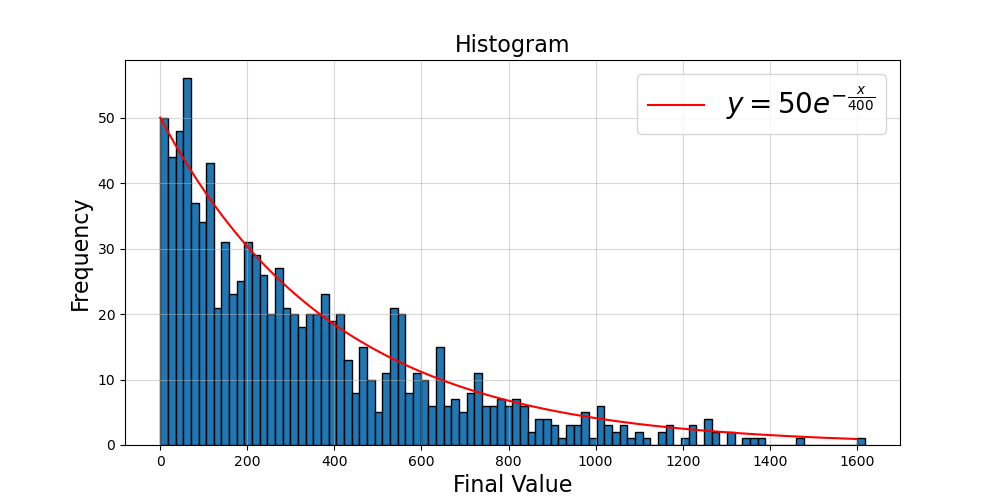
\includegraphics[width=5in]{hist.png}
   \label{myfig}
\end{figure}

Our histogram has 1000 data points with 92 bins (92 divides 2024). We can see our histogram has a right skew as we have more heavily-weight data points on the right of our mean. Thus our ratio of about $\frac{1}{6}$ is also skewed to the right. We can also see our mode is below our average. On our graph, we also have $y = 50e^{-\frac{x}{400}}$ to show a similar graph.

We reach our second \keyword{Conjecture} conjecture: The distribution follows an exponential decay graph. However, we immediately \keyword{Stuck} get stuck and even trying a smaller hat with a larger amount of data points we see more a positive skewed graph than exponential. The below graph showing 10,000 data points for a hat of size $n = 100$. 

\begin{figure}[h] 
   \centering
   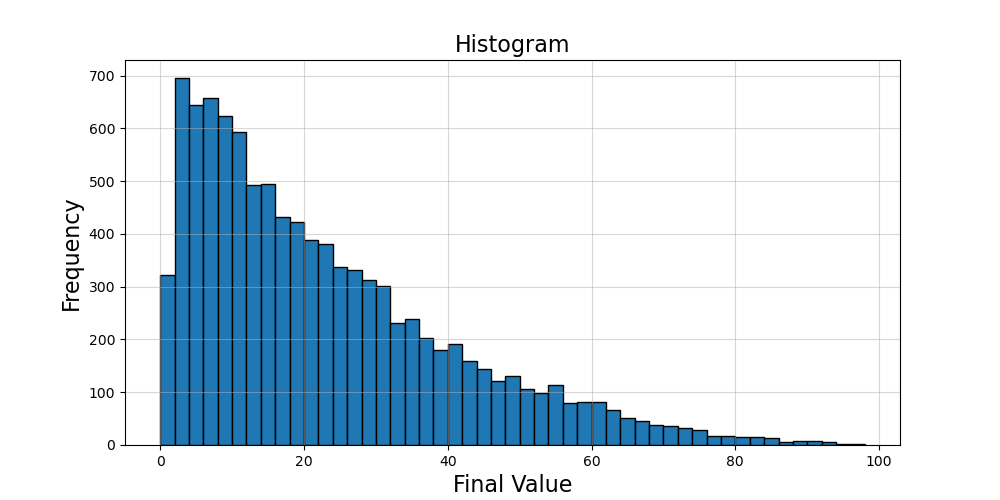
\includegraphics[width=5in]{hist2.png}
   \label{myfig}
\end{figure}

%-----------------------------------------------------------------------------------------------------------

\section{Review} %------------------------------------------------------------------------------------------



Reviewing our initial questions, \keyword{Check} we found that our final value will always be even, within the range of 0 to 2024, with a mean of  $\approx337$. It is impossible to obtain an odd number under our initial conditions. We also found that, yes, our starting parameters does indeed affect our final values. Based on Table 1, we found there are 4 classes, but two are actually the same as both odd cases give the same values. Thus we get 3 unique cases depending on $n \text{ mod } 4$. We were also able to show in our histograms that there was right-skewness and that higher numbers were less likely to occur. 

Reviewing the work done, \keyword{Reflect} discovering the pattern was a major milestone as it provided necessary information to answer our beginning questions. This highlights the benefits on systematic specialisation. Justifying my first conjecture was also satisfying to explain why we only get odd or even numbers. I had to be extra careful to state the number of odd valued pieces of paper as that number could be odd or even. The help of the table shows how depending on the combination, they can either reduce the number of odd or even valued paper. Similar to the poison, water, antidote game we played in class. 

The biggest issue that I faced was the final part of the attack. With my limited statistics knowledge, I was unable to determine what distribution our histogram would conform to. I did not have enough justification to say that it is in fact a decay function or a positive skew graph. Despite this setback, I believe that I have explored our hat of 2024 to a appropriate degree. 

Similar to the previous assignment, Python \keyword{Reflect} was vital in calculating and plotting large quantities of data. Again, similarly to previous assignments, we can't use it to explore extremely large values of $n$ as my code is not close to being optimised for such tasks. Even the programming language, Python, may not be the best for the task as other languages may be better/more optimised. I also don't have a full understanding of some libraries, which became a issue when I realised I couldn't fit a skewed graph onto my histogram but I was still explain my thoughts despite this. Lastly, dealing with random numbers, it would have been a wise idea to use a seed on certain parts. This would be so I am able to test my code multiple times without it changing.

There are a few ways to \keyword{Extend} explore this further:
\begin{itemize}
    \item Hats of different sizes and numbers
    \begin{itemize}
        \item Instead of starting at 1 and ending at 2024, we could start at any $x$ and end at $y$. $[x, y] \text{ s.t. } x, y \in \mathbb{N}$ 
        \item Having different step values. All odd or even numbers between 1 and 2024 will alter the final value. We could choose every third, fourth, fifth, \dots, $n^{\text{th}}$ number.
        \item We could move away from the natural numbers and have rationals, irrationals and even complex.
    \end{itemize}
    \item Have the first number minus the second; this gives the possibility of negative numbers.
    \item Continuing the above idea, we could change to any binary operation to generate our new number.
\end{itemize}

We will try exploring what happens when changing our  \keyword{Extend} initial condition. We explore with small hats of \keyword{Specialise} \{1, 2,\dots, 10\}, \{11, 12,\dots, 20\}, and  \{21, 22,\dots, 30\}, we find their averages to be 2.966, 5.57, 5.7916. Finding more averages for the group of hats \{31, 32,\dots, 40\}, \{41, 42,\dots, 50\}, and  \{51, 52,\dots, 60\}, we get 5.8838, 5.781, and 5.8286 respectively. We see that for the first hat, we get an average of about 3 but for the subsequent hats we have averages of around 5.7. We know our initial hat has possible values of {1, 3, 5, 7, 9} but for our second hat, we now get  {1, 3, 5, 7, \dots, 15, 17, 19}. An interesting thing to note is that our latter  four hats only have possible values of {1, 3, 5, \dots, 21, 23, 25}.  Further exploration could determine that this holds generally. 

Lastly, we attempt to just use difference instead of absolute difference. We now get an average that hovers around 0 but has a high variance. This is because our final value can quite often be in the tens of thousands in both the positive and negative directions. 


\section*{Supplementary material}
The code for this assignment can be found on my GitHub page:  \url{https://github.com/LazyTim/MA3K7/blob/main/MA3K7%20-%20Assignment%203.ipynb}.

\end{document}
